\documentclass[11pt]{article}

\usepackage{fullpage}
\usepackage{graphicx}
\usepackage{amsmath}
\usepackage{amssymb}
\usepackage{amsthm}
\usepackage{enumitem}
\usepackage{tikz}
\usepackage{subcaption}
\usepackage{caption}
\usetikzlibrary{automata,positioning}

\parindent0in
\pagestyle{plain}
\thispagestyle{plain}

%% UPDATE MACRO DEFINITIONS %%
\newcommand{\myname}{Bishwa Nath Silwal}
\newcommand{\assignment}{Assignment I}
\newcommand{\duedate}{September 14, 2017}

\usepackage{etoolbox}% http://ctan.org/pkg/etoolbox
\usepackage{enumitem}% http://ctan.org/pkg/enumitem
\newcounter{mycount} \renewcommand{\themycount}{\arabic{mycount}}%
\AtBeginEnvironment{enumerate}{\stepcounter{mycount}}% Increment m
\setlist[enumerate]{label=\themycount.\arabic*,ref=\themycount.\arabic*}
%% DO NOT CHANGE ANYTHING BELOW THIS LINE %%

\begin{document}

\textbf{Howard University}\hfill\textbf{\myname}\\[0.01in]
\textbf{CS -- Theory of Computation}\hfill\textbf{\assignment}\\[0.01in]
\textbf{Prof.\ Chunmei Liu}\hfill\textbf{\duedate}\\
\smallskip\hrule\bigskip


\begin{enumerate}\bfseries
	\item [1.1] 
	      	      
	      \begin{enumerate}[label=(\alph*)]
	      	\item What is the start state? \\
	      	      {\normalfont $q_1$ is the start state in both DFAs}
	      	\item What is the set of accept states? \\
	      	      {\normalfont $F_1 = \{q_2\}$ and $F_2 = \{q_1, q_4\}$}
	      	\item What sequence of states does the machine go through on input aabb? \\
	      	      {\normalfont For $M_1$, the machine goes through $q_1$, $q_2$, $q_3$, $q_1$ , $q_1$.} \\
	      	      {\normalfont For $M_2$, the machine goes through $q_1$, $q_1$, $q_1$, $q_2$ , $q_4$.}
	      	\item Does the machine accept the string aabb? \\
	      	      {\normalfont $M_1$ does not accept the string aabb while $M_2$ accepts it because the end state is not the accept state in $M_1$, while in $M_2$, the end state is the accept state.} 
	      	\item Does the machine accept the string $\epsilon$ ? \\
	      	      {\normalfont $M_1$ doesnt accept the string $\epsilon$ but $M_2$ does since the start state of $M_2$ is also the accepting state.}
	      \end{enumerate}
	      	      	
	\item [1.2]Give the formal descriptions of the machine $M_1$ and $M_2$ pictured in Exercise 1.1.
	      $M_1 = \{ \{q_1, q_2, q_3\} , \{a,b\}, \delta, q_1, \{q_3\}\}$ \\
	      {\normalfont where the transition function $\delta$ is given by the following table:} \\\
	      \begin{center}
	      	\begin{tabular}{|c |c |c|}
	      		\hline
	      		State & a     & b     \\
	      		\hline 
	      		$q_1$ & $q_2$ & $q_1$ \\ 
	      		\hline
	      		$q_2$ & $q_3$ & $q_3$ \\
	      		\hline
	      		$q_3$ & $q_2$ & $q_1$ \\
	      		\hline
	      	\end{tabular}
	      \end{center}
	      	        		
	      	        		
	      $M_2 = \{ \{q_1, q_2, q_3, q_4\} , \{a,b\}, \delta, q_1, \{q_1, q_4\}\}$ \\
	      {\normalfont where the transition function $\delta$ is given by the following table:} \\
	      \begin{center}
	      	\begin{tabular}{|c |c |c|}
	      		\hline
	      		State & a     & b     \\
	      		\hline
	      		$q_1$ & $q_1$ & $q_2$ \\ 
	      		\hline
	      		$q_2$ & $q_3$ & $q_4$ \\
	      		\hline
	      		$q_3$ & $q_2$ & $q_1$ \\ 
	      		\hline
	      		$q_4$ & $q_3$ & $q_4$ \\
	      		\hline
	      	\end{tabular}
	      \end{center}
	      	        		
	\item [1.3] The formal description of a DFA M is
	      $\{ \{q_1, q_2, q_3, q_4, q_5\} , \{u,d\}, \delta, q_3, \{q_3\}\}$
	      where $\delta$ is given by the following table. Give the state diagram of this machine: \\
	      	        
	      {\normalfont The state diagram of the machine is as follows:}
	      	        
	      	        
	      \begin{center}
	      	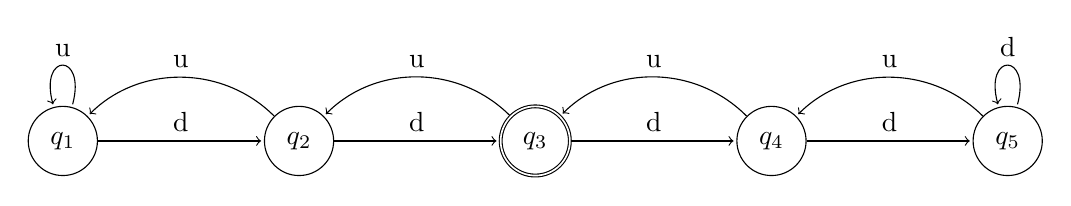
\begin{tikzpicture}[shorten >=1pt,node distance=3cm,on grid,auto, every loop/.style={<-,shorten <=1pt}]
	      			      		  
	      		\node[state] (q_1)   {$q_1$}; 
	      		\node[state] (q_2) [right=of q_1] {$q_2$};
	      		\node[state,accepting] (q_3) [right=of q_2] {$q_3$};
	      		\node[state] (q_4) [right=of q_3] {$q_4$};
	      		\node[state] (q_5) [right=of q_4] {$q_5$}; 
	      		\path[->] 
	      		(q_1) edge node {d} (q_2)
	      		edge [loop above] node {u} ()
	      		(q_2) edge node  {d} (q_3)
	      		edge [bend right=45] node [swap] {u} (q_1)
	      		(q_3) edge node  {d} (q_4)
	      		edge [bend right=45] node [swap] {u} (q_2)
	      		(q_4) edge node  {d} (q_5)
	      		edge [bend right=45] node [swap] {u} (q_3)
	      		(q_5) edge [loop above] node {d} ()
	      		edge [bend right=45] node [swap] {u} (q_4);
	      	\end{tikzpicture}
	      \end{center}
	      	         	
	\item [1.4] Hello
	      	      
		\begin{enumerate}
	      	\item [(a)] {\normalfont Here, the two DFAs are:}
	      	      \begin{figure}[hbp]
	      	      	\centering
	      	      		      	    
	      	      	\begin{subfigure}[apple] {0.4\textwidth}  	      	
	      	      		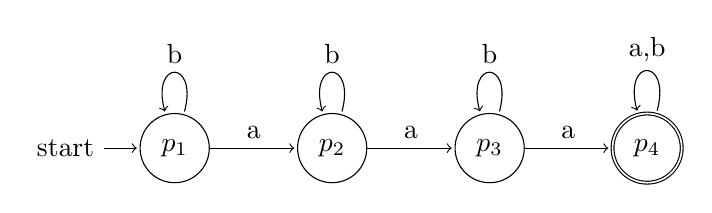
\begin{tikzpicture}[shorten >=1pt,node distance=2cm,on grid,auto, every loop/.style={<-,shorten <=1pt}]
	      	      			\node[state,initial] (p_1)   {$p_1$}; 
	      	      			\node[state] (p_2) [right=of p_1] {$p_2$}; 
	      	      			\node[state] (p_3) [right=of p_2] {$p_3$};  
	      	      			\node[state, accepting] (p_4) [right=of p_3] {$p_4$}; 
	      	      			\path[->] 
	      	      			(p_1) 	edge node {a} (p_2)
	      	      					edge [loop above] node {b} ()
	      	      			(p_2) 	edge node {a} (p_3)
			      	      			edge [loop above] node {b} ()
	      	      			(p_3) 	edge node {a} (p_4)
								    edge [loop above] node {b} ()  	      			
	      	      			(p_4)	edge [loop above] node {a,b} ();
	      	      				      	      			
	      	      		\end{tikzpicture}	
	      	      		\caption{\{$w | w$ has at least three a's\}}
	      	      	\end{subfigure}\hfill
	      	      	\begin{subfigure}[apple] {0.4\textwidth}  	      	
	      	      		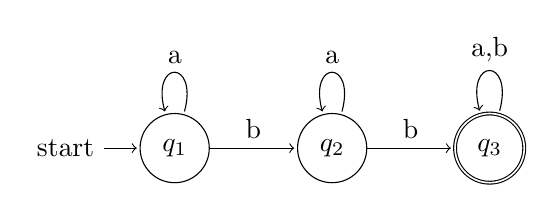
\begin{tikzpicture}[shorten >=1pt,node distance=2cm,on grid,auto, every loop/.style={<-,shorten <=1pt}]
	      	      			\node[state,initial] (q_1)   {$q_1$}; 
	      	      			\node[state] (q_2) [right=of q_1] {$q_2$}; 
	      	      			\node[state, accepting] (q_3) [right=of q_2] {$q_3$};
	      	      			\path[->] 
	      	      			(q_1) 	edge node {b} (q_2)
	      	      					edge [loop above] node {a} ()
	      	      			(q_2) 	edge node {b} (q_3)
			      	      			edge [loop above] node {a} ()
	      	      			(q_3) 	edge [loop above] node {a,b} ();
	      	      				      	      			
	      	      		\end{tikzpicture}	
	      	      		\caption{\{$w | w$ has at least two b's\}}
	      	      	\end{subfigure}\\
	      	      \end{figure}
	      	      
	      	      
	      	      {\normalfont The combined DFA is as follows:}
	      	      
	      	      \begin{figure} [hbp]
	      	     
	      	     \begin{center}
	      	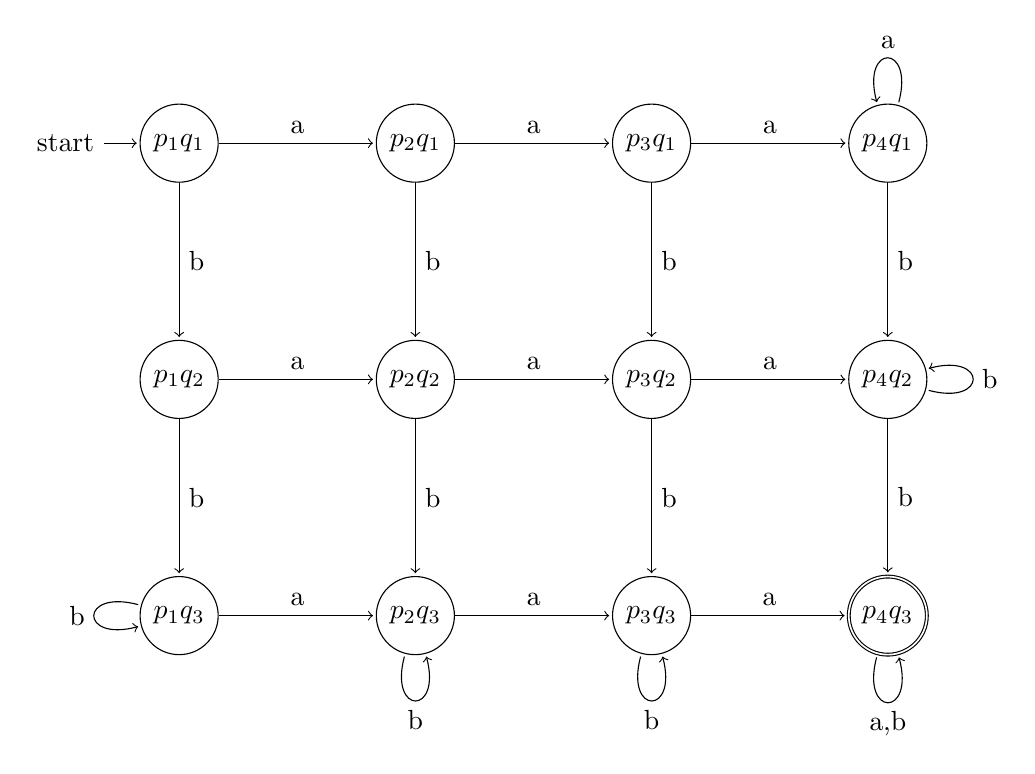
\begin{tikzpicture}[shorten >=1pt,node distance=3cm,on grid,auto, every loop/.style={<-,shorten <=1pt}]
	      			      		  
	      		\node[state,initial] (a)   {$p_1q_1$}; 
	      		\node[state] (b) [right=of a] {$p_2q_1$};
	      		\node[state] (c) [right=of b] {$p_3q_1$};
	      		\node[state] (d) [right=of c] {$p_4q_1$};
	      		\node[state] (e) [below=of a] {$p_1q_2$};
	      		\node[state] (f) [right=of e] {$p_2q_2$};
	      		\node[state] (g) [right=of f] {$p_3q_2$};
	      		\node[state] (h) [right=of g] {$p_4q_2$};
	      		\node[state] (i) [below=of e] {$p_1q_3$};
	      		\node[state] (j) [right=of i] {$p_2q_3$};
	      		\node[state] (k) [right=of j] {$p_3q_3$};
	      		\node[state, accepting] (l) [right=of k] {$p_4q_3$};
	      		
	      		\path[->] 
	      	      	(a) 	edge node {a} (b)
							edge node {b} (e)
					(b) 	edge node {a} (c)
							edge node {b} (f)
					(c) 	edge node {a} (d)
							edge node {b} (g)
					(d) 	edge [loop above] node {a} ()
							edge node {b} (h)
					(e) 	edge node {a} (f)
							edge node {b} (i)
					(f) 	edge node {a} (g)
							edge node {b} (j)
					(g) 	edge node {a} (h)
							edge node {b} (k)
					(h) 	edge [loop right] node {b} ()
							edge node {b} (l)
					(i) 	edge [loop left] node {b} ()
							edge node {a} (j)
					(j) 	edge [loop below] node {b} ()
							edge node {a} (k)
					(k) 	edge [loop below] node {b} ()
							edge node {a} (l)
					(l) 	edge [loop below] node {a,b} ();
							
	      	\end{tikzpicture}
	      	
	      	\caption{Combined DFA of the two Languages}
	      \end{center}
	      \end{figure}
	      
	      
	    \clearpage
	      \item [(c)] {\normalfont Here, the two DFAs are:}
	       \begin{figure}[hbp]	      	      		      	    
	      	      	\begin{subfigure}[apple] {0.5\textwidth}  	      	
	      	      		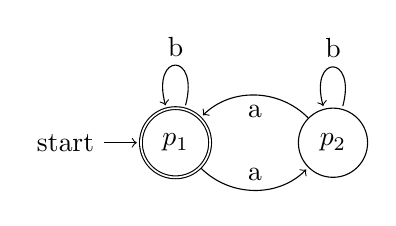
\begin{tikzpicture}[shorten >=1pt,node distance=2cm,on grid,auto, every loop/.style={<-,shorten <=1pt}]
	      	      			\node[state,initial, accepting] (p_1)   {$p_1$}; 
	      	      			\node[state] (p_2) [right=of p_1] {$p_2$}; 
	      	      			\path[->] 
	      	      			(p_1) 	edge [bend right=45] node {a} (p_2)
	      	      					edge [loop above] node {b} ()
	      	      			(p_2) 	edge [bend right=45] node  {a} (p_1)
			      	      			edge [loop above] node {b} ();
	      	      			
	      	      				      	      			
	      	      		\end{tikzpicture}	
	      	      		\caption{\{$w | w$ has at least three a's\}}
	      	      	\end{subfigure}\hfill
	      	      	\begin{subfigure}[apple] {0.5\textwidth}  	      	
	      	      		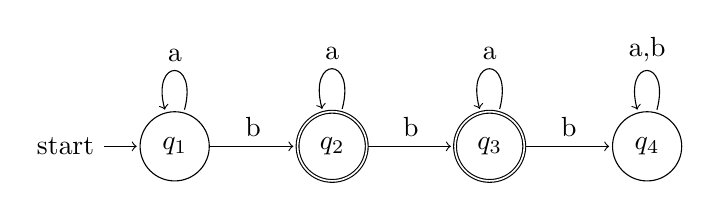
\begin{tikzpicture}[shorten >=1pt,node distance=2cm,on grid,auto, every loop/.style={<-,shorten <=1pt}]
	      	      			\node[state,initial] (q_1)   {$q_1$}; 
	      	      			\node[state, accepting] (q_2) [right=of q_1] {$q_2$}; 
	      	      			\node[state, accepting] (q_3) [right=of q_2] {$q_3$};
	      	      			\node[state] (q_4) [right=of q_3] {$q_4$};
	      	      			
	      	      			\path[->] 
	      	      			(q_1) 	edge node {b} (q_2)
	      	      					edge [loop above] node {a} ()
	      	      			(q_2) 	edge node {b} (q_3)
			      	      			edge [loop above] node {a} ()
							(q_3) 	edge node {b} (q_4)	
			      	      			edge [loop above] node {a} ()
	      	      			(q_4) 	edge [loop above] node {a,b} ();
	      	      			
	      	      				      	      			
	      	      		\end{tikzpicture}	
	      	      		\caption{\{$w | w$ has at one or two b's\}}
	      	      	\end{subfigure}\\
	      	      \end{figure}
	      	      
	      	      {\normalfont The combined DFA is as follows:}
	      	      
	      	      \begin{figure} [hbp]
	      	     
	      	     \begin{center}
	      	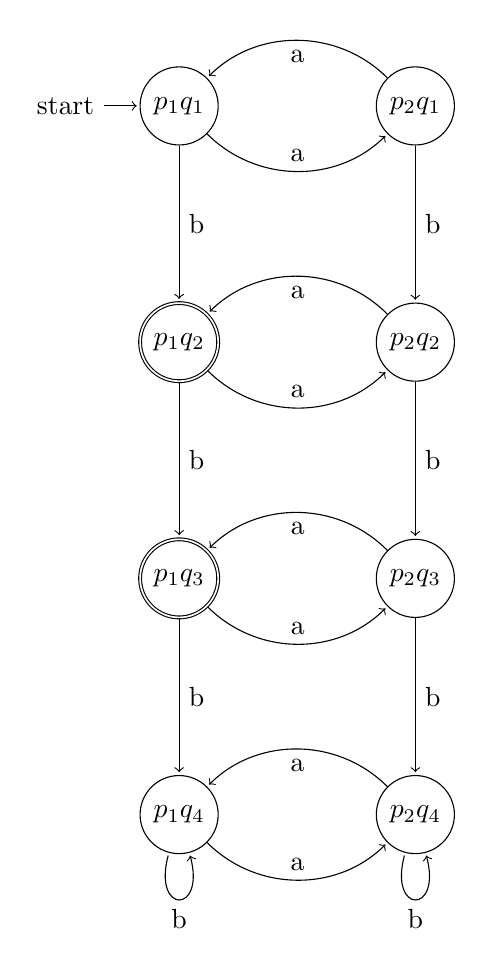
\begin{tikzpicture}[shorten >=1pt,node distance=3cm,on grid,auto, every loop/.style={<-,shorten <=1pt}]
	      			      		  
	      		\node[state,initial] (a)   {$p_1q_1$}; 
	      		\node[state] (b) [right=of a] {$p_2q_1$};
	      		
	      		\node[state, accepting] (e) [below=of a] {$p_1q_2$};
	      		\node[state] (f) [right=of e] {$p_2q_2$};
	      		
	      		\node[state, accepting] (i) [below=of e] {$p_1q_3$};
	      		\node[state] (j) [right=of i] {$p_2q_3$};
	      		
	      		\node[state] (k) [below=of i] {$p_1q_4$};
	      		\node[state] (l) [right=of k] {$p_2q_4$};
	      		
	      		
	      		\path[->] 
	      	      	(a) 	edge [bend right=45] node {a} (b)
							edge node {b} (e)
					(b) 	edge [bend right=45] node {a} (a)
							edge node {b} (f)
					
					(e) 	edge [bend right=45] node {a} (f)
							edge node {b} (i)
					(f) 	edge [bend right=45] node {a} (e)
							edge node {b} (j)
					
					
					(i) 	edge [bend right=45] node {a} (j)
							edge node {b} (k)
					(j) 	edge [bend right=45] node {a} (i)
							edge node {b} (l)
							
					(k) 	edge [loop below] node {b} ()
							edge [bend right=45] node {a} (l)
					(l) 	edge [loop below] node {b} ()
							edge [bend right=45] node {a} (k);
							
	      	\end{tikzpicture}
	      	
	      	\caption{Combined DFA of the two Languages}
	      \end{center}
	      \end{figure}
	      
	      \clearpage
	      \item [(e)] {\normalfont The two DFAs are}
	      
	      \begin{figure}[hbp]	      	      		      	    
	      	      	\begin{subfigure}[apple] {0.5\textwidth}  	      	
	      	      		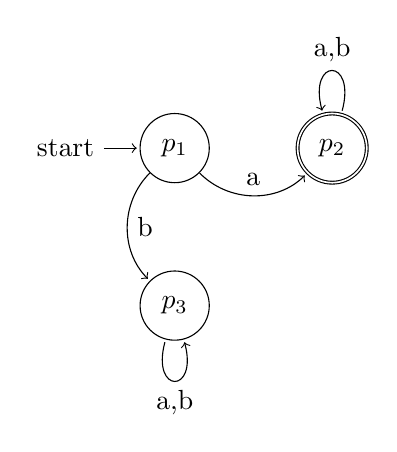
\begin{tikzpicture}[shorten >=1pt,node distance=2cm,on grid,auto, every loop/.style={<-,shorten <=1pt}]
	      	      			\node[state, initial] (p_1)   {$p_1$}; 
	      	      			\node[state, accepting] (p_2) [right=of p_1] {$p_2$}; 
	      	      			\node[state] (p_3) [below=of p_1] {$p_3$};
	      	      			
	      	      			\path[->] 
	      	      			(p_1) 	edge [bend right=45] node {a} (p_2)
	      	      					edge [bend right=45] node {b} (p_3)
	      	      			(p_2) 	edge [loop above] node {a,b} ()
							(p_3) 	edge [loop below] node {a,b} ();
	      	      			
	      	      				      	      			
	      	      		\end{tikzpicture}	
	      	      		\caption{\{$w | w$ starts with an a\}}
	      	      	\end{subfigure}\hfill
	      	      	\begin{subfigure}[apple] {0.5\textwidth}  	      	
	      	      		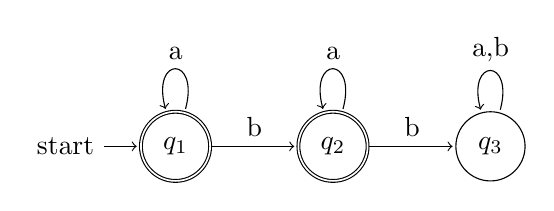
\begin{tikzpicture}[shorten >=1pt,node distance=2cm,on grid,auto, every loop/.style={<-,shorten <=1pt}]
	      	      			\node[state,initial, accepting] (q_1)   {$q_1$}; 
	      	      			\node[state, accepting] (q_2) [right=of q_1] {$q_2$}; 
	      	      			\node[state] (q_3) [right=of q_2] {$q_3$};
	      	      		
	      	      			
	      	      			\path[->] 
	      	      			(q_1) 	edge node {b} (q_2)
	      	      					edge [loop above] node {a} ()
	      	      			(q_2) 	edge node {b} (q_3)
			      	      			edge [loop above] node {a} ()
							(q_3) 	edge [loop above] node {a,b} ();
	      	    
	      	      			
	      	      				      	      			
	      	      		\end{tikzpicture}	
	      	      		\caption{\{$w | w$ has at most one b\}}
	      	      	\end{subfigure}\\
	      	      \end{figure}
	      
	       \clearpage
	       
	      \item [(f)] {\normalfont The two DFAs are} 
	      
	      \begin{figure}[hbp]	      	      		      	    
	      	      	\begin{subfigure}[apple] {0.5\textwidth}  	      	
	      	      		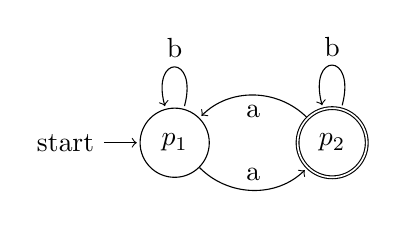
\begin{tikzpicture}[shorten >=1pt,node distance=2cm,on grid,auto, every loop/.style={<-,shorten <=1pt}]
	      	      			\node[state,initial] (p_1)   {$p_1$}; 
	      	      			\node[state, accepting] (p_2) [right=of p_1] {$p_2$}; 
	
	      	      		
	      	      			
	      	      			\path[->] 
	      	      			(p_1) 	edge [bend right=45] node {a} (p_2)
	      	      					edge [loop above] node {b} ()
	      	      			(p_2) 	edge [bend right=45] node {a} (p_1)
			      	      			edge [loop above] node {b} ();
			      	      			
	      	      				
	      	      		\end{tikzpicture}	
	      	      		\caption{\{$w | w$ has an odd number of a's\}}
	      	      	\end{subfigure}\hfill
	      	      	\begin{subfigure}[apple] {0.5\textwidth}  	      	
	      	      		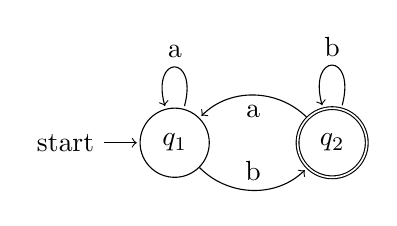
\begin{tikzpicture}[shorten >=1pt,node distance=2cm,on grid,auto, every loop/.style={<-,shorten <=1pt}]
	      	      			\node[state,initial] (q_1)   {$q_1$}; 
	      	      			\node[state, accepting] (q_2) [right=of q_1] {$q_2$}; 
	
	      	      		
	      	      			
	      	      			\path[->] 
	      	      			(q_1) 	edge [bend right=45] node {b} (q_2)
	      	      					edge [loop above] node {a} ()
	      	      			(q_2) 	edge [bend right=45] node {a} (q_1)
			      	      			edge [loop above] node {b} ();

	      	    
	      	      			
	      	      				      	      			
	      	      		\end{tikzpicture}	
	      	      		\caption{\{$w | w$ ends with b\}}
	      	      	\end{subfigure}\\
	      	      \end{figure}
	      
			  
	      	      {\normalfont The combined DFA is as follows:}
	      	      
	      	      \begin{figure} [hbp]
	      	     
	      	     \begin{center}
	      	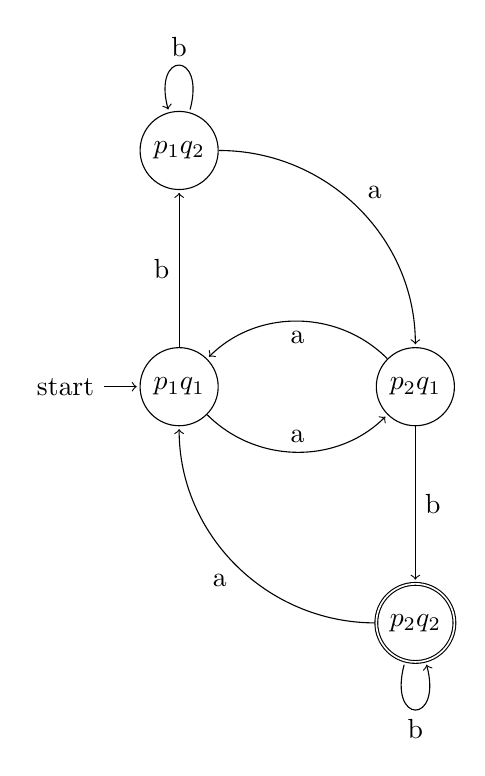
\begin{tikzpicture}[shorten >=1pt,node distance=3cm,on grid,auto, every loop/.style={<-,shorten <=1pt}]
	      			      		  
	      		\node[state,initial] (a)   {$p_1q_1$}; 
	      		\node[state] (b) [right=of a] {$p_2q_1$};
	      		
	      		\node[state] (e) [above=of a] {$p_1q_2$};
	      		\node[state, accepting] (f) [below=of b] {$p_2q_2$};
	      		
	      		
	      		
	      		\path[->] 
	      	      	(a) 	edge [bend right=45] node {a} (b)
							edge node {b} (e)
					(b) 	edge node {b} (f)
							edge [bend right=45] node {a} (a)
					
					(e) 	edge [bend left=45] node {a} (b)
							edge [loop above] node {b} ()
					(f) 	edge [bend left=45] node {a} (a)
							edge [loop below] node {b} ();
	      	\end{tikzpicture}
	      	
	      	\caption{Combined DFA of the two Languages}
	      \end{center}
	      \end{figure}

		\clearpage
	      \item [(g)] {\normalfont The two DFAs are} 
	      
	      \begin{figure}[hbp]	      	      		      	    
	      	      	\begin{subfigure}[apple] {0.5\textwidth}  	      	
	      	      		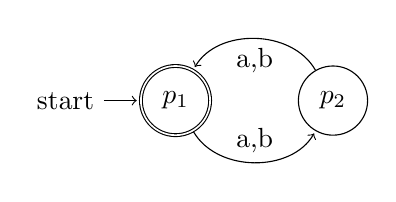
\begin{tikzpicture}[shorten >=1pt,node distance=2cm,on grid,auto, every loop/.style={<-,shorten <=1pt}]
	      	      			\node[state,initial, accepting] (p_1)   {$p_1$}; 
	      	      			\node[state] (p_2) [right=of p_1] {$p_2$}; 
	
	      	      		
	      	      			
	      	      			\path[->] 
	      	      			(p_1) 	edge [bend right=60] node {a,b} (p_2)
	      	      			(p_2) 	edge [bend right=60] node {a,b} (p_1);
			      	      			      	      				
	      	      		\end{tikzpicture}	
	      	      		\caption{\{$w | w$ has even length b\}}
	      	      	\end{subfigure}\hfill
	      	      	\begin{subfigure}[apple] {0.5\textwidth}  	      	
	      	      		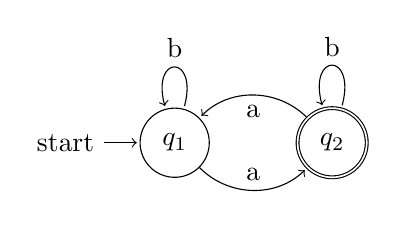
\begin{tikzpicture}[shorten >=1pt,node distance=2cm,on grid,auto, every loop/.style={<-,shorten <=1pt}]
	      	      			\node[state,initial] (q_1)   {$q_1$}; 
	      	      			\node[state, accepting] (q_2) [right=of q_1] {$q_2$}; 
	
	      	      		
	      	      			
	      	      			\path[->] 
	      	      			(q_1) 	edge [bend right=45] node {a} (q_2)
	      	      					edge [loop above] node {b} ()
	      	      			(q_2) 	edge [bend right=45] node {a} (q_1)
			      	      			edge [loop above] node {b} ();
			      	      			
	      	      				
	      	      		\end{tikzpicture}	
	      	      		\caption{\{$w | w$ has an odd number of a's\}}
	      	      	\end{subfigure}\\
	      	      \end{figure}
	      
			  
	      	      {\normalfont The combined DFA is as follows:}
	      	      
	      	      \begin{figure} [hbp]
	      	     
	      	     \begin{center}
	      	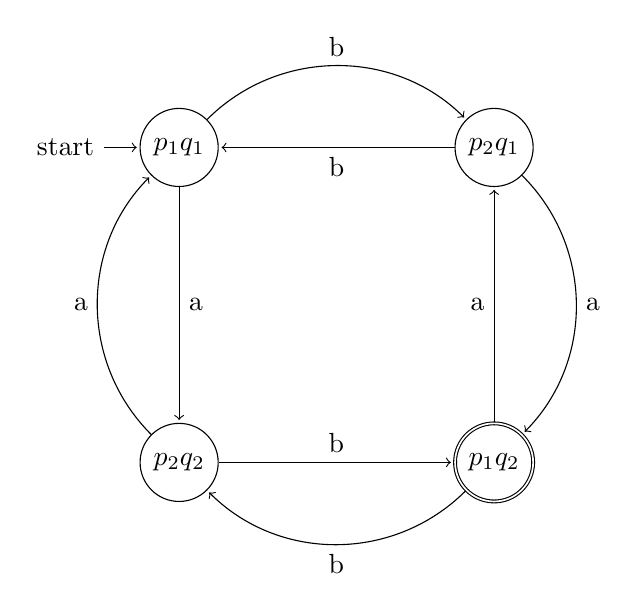
\begin{tikzpicture}[shorten >=1pt,node distance=4cm,on grid,auto, every loop/.style={<-,shorten <=1pt}]
	      			      		  
	      		\node[state,initial] (a)   {$p_1q_1$}; 
	      		\node[state] (b) [right=of a] {$p_2q_1$};
	      		
	      		\node[state, accepting] (e) [below=of b] {$p_1q_2$};
	      		\node[state] (f) [below=of a] {$p_2q_2$};
	      		
	      		
	      		
	      		\path[->] 
	      	      	(a) 	edge node {a} (f)
							edge [bend left=45] node {b} (b)
							
					(b) 	edge  node {b} (a)
							edge [bend left=45] node {a} (e)
					
					(f) 	edge node {b} (e)
							edge [bend left=45] node {a} (a)

					(e) 	edge [bend left=45] node {b} (f)
							edge  node {a} (b);
	      	\end{tikzpicture}
	      	
	      	\caption{Combined DFA of the two Languages}
	      \end{center}
	      \end{figure}
	      
	      \end{enumerate}
      
	      
	\item [1.6] 
	      		\begin{enumerate}
	      			\item [(a)] {\normalfont The two DFAs are} 
	      
	      		\end{enumerate}
	      	     
\end{enumerate} 
 
\end{document}
